
\section{Requirements specification for Main Application Module}\label{Requirements specifications for Main Application Module}
\subsection{General Definition}\label{GeneralDefinition main}
Main Application Module (MAM) is an application, which responsible for management N2Sky system. It embeds:
\begin{itemize}
\item Model Repository 
\item Neural Network Repository 
\item N2Sky Main Dashboard.
\end{itemize}

MAM is a core component of the N2Sky platform. From this component, users can feel the power of the N2Sky system and try out the whole functionality of it. The MAM, as well as other N2Sky components, is possible to use on any device because it supports responsive design. 

\subsection{Affected users}\label{Affected users MAM}
The MAM has one User Interface but users can use it diverse. Only users, which the main function is within MAM can operate this module on their own purpose. Following types of users have this kind of the main function:

\begin{itemize}
\item \emph{Arbitrary User.} The main function of the arbitrary user is to learn about neural networks or try out his knowledge in this field. The typical use case is when the user logs in from the mobile device like smartphone all tablet and search something in repositories. This user copy existing neural networks or trained models into own project and perform some operations on it.  A detailed description is in \autoref{User Roles}. 
\item \emph{Neural Network Engineer User.} This kind of user normally uses Desktop version of N2Sky, but he can also use the mobile version because all functionalities are also available there. The user creates own neural network from existing paradigm, but he also can act as an Arbitrary User.  A detailed description is in \autoref{User Roles}. 
\item \emph{Contributor User.} The Contributor uses N2Sky MAM component mostly for an easier way to check his own neural network paradigm. Since this user can fully use N2Sky open API, UI for him is just for the quick check. The UI is available also in the mobile version, that is why Contributor can observe his neural networks behavior directly from the mobile device in any place. A detailed description is in \autoref{User Roles}. 
\item \emph{System Administrator.} His main function is on AM module, but since he is also the administrator of the N2Sky MAM he can see all processes of other users. This user can shadow any other user in order to see what is happening in particular user dashboard.  A detailed description is in \autoref{User Roles}. 
\end{itemize}

\subsection{N2Sky Dashboard}\label{N2Sky Dashboard}
The N2Sky dashboard is the central component of the MAM module. The dashboard gives brief information about available tools, user's projects and user's neural networks. Every dashboard is unique for every user, namely, the content always differs. As it is displayed in figure \ref{fig:n2skymaindashboard}, the dashboard gives a full overview of the components from one page.

\begin{figure}[htbp]
\begin{center}
  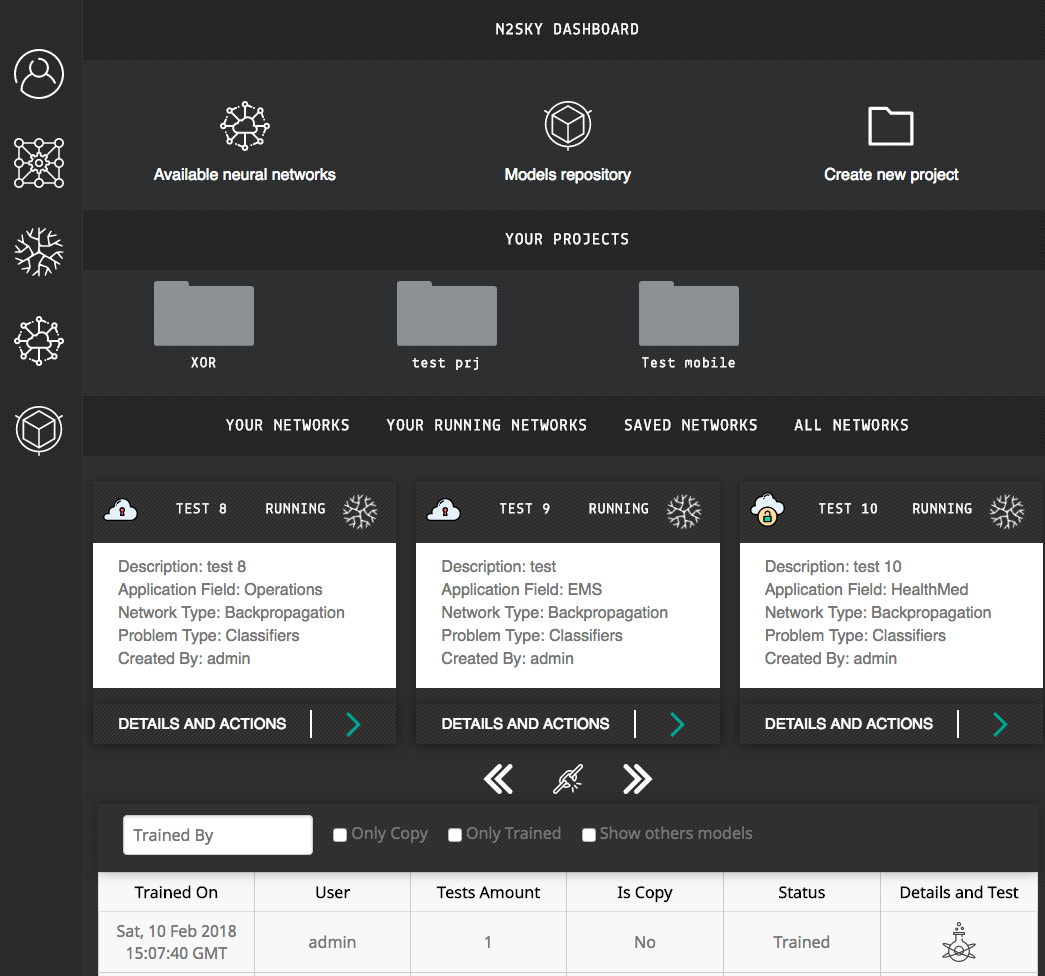
\includegraphics[width=\linewidth]{components/5/img/n2sky_main_dashboard.png}
  \caption{N2Sky User Dashboard}
  \label{fig:n2skymaindashboard}
\end{center}
\end{figure}

The N2Sky dashboard contains following components:
\begin{itemize}
\item Available tools
\item The user projects
\item The user neural networks 
\item The user trained models
\end{itemize}

The dashboard is available under following URL path:
 \begin{lstlisting}
    <host>/cloud
\end{lstlisting}

\subsubsection{Available tools}

\begin{figure}[htbp]
\begin{center}
  
\includegraphics[scale=0.5]{components/5/img/n2sky_tools.png}
  \caption{N2Sky Main Module. Available user tools}
  \label{fig:n2sky_tools}
\end{center}
\end{figure}

In figure \ref{fig:n2sky_tools} the available tools component is displayed in a horizontal layout. Every item has an SVG icon and caption under it. The tools contain following functionalities: 
\begin{itemize}
\item \emph{Available neural network.} Reference to the available repositories view.  
\item \emph{Model repository.} Reference to the model repository view.
\item \emph{Create a new project.} On click of this time the popup window will be initialized as it displayed in figure \ref{fig:popupcreatenewproject}.


\begin{figure}[htbp]
\begin{center}
  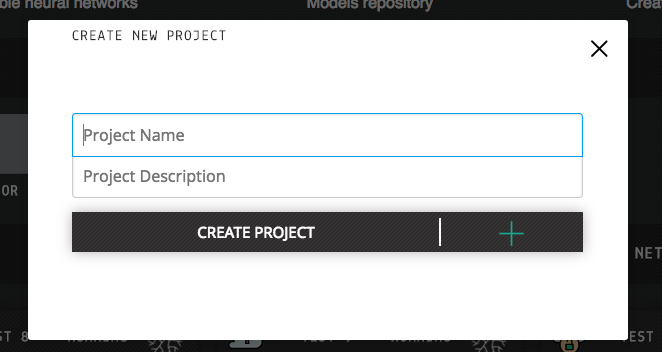
\includegraphics[scale=0.5]{components/5/img/popupcreatenewproject.png}
  \caption{N2Sky Main Module. Create New Project Popup}
  \label{fig:popupcreatenewproject}
\end{center}
\end{figure}


The following popup modal window contains components:
\begin{itemize}
\item \emph{Project Name} field, which represents a short title of the project.
\item \emph{Project Description} field with a short description of the project, which will be used for the semantic search.  
\item \emph{Create Project} button, which created a project with filled up form.
\end{itemize}

After creating the project it will automatically appear in the dashboard. 

\end{itemize}

\subsubsection{User projects}

User projects is a grid with projects. Every project is represented as a folder with a caption under it as it displayed in figure \ref{fig:n2sky_dashboard_projects}. On click, the user will be redirected to the particular project. 

\begin{figure}[htbp]
\begin{center}
  
\includegraphics[scale=0.5]{components/5/img/n2sky_dashboard_projects.png}
  \caption{N2Sky Main Module. User projects grid}
  \label{fig:n2sky_dashboard_projects}
\end{center}
\end{figure}

 \subsubsection{The user neural networks and models overview}
 
 The component is displaying the neural networks of the user, which either created from paradigm or own contributed neural networks. The component contains following subcomponents:
 \begin{itemize}
\item \emph{Neural networks filtering bar.}
The filtering bar is a navigation as well as neural networks filtering subcomponent as is shown in figure \ref{fig:n2sky_filtering_bar}. The subcomponent allows the user to filter through neural networks depending on permissions. 

\begin{figure}[htbp]
\begin{center}
  
\includegraphics[scale=0.5]{components/5/img/n2sky_filtering_bar.png}
  \caption{N2Sky Main Module. Neural networks filtering bar.}
  \label{fig:n2sky_filtering_bar}
\end{center}
\end{figure}

The following filters are available: 
\begin{itemize}
\item \emph{Your networks.} The filter shows the running and not running neural networks of the logged in user. 
\item \emph{Your running networks.} The representation only of the user's running neural networks.
\item \emph{Saved networks.} Only saved neural networks of the users. The list will show the saved neural networks across all projects of the user.
\item \emph{All Networks}. List of all networks on the N2Sky. This filter is available only for the system administrator.
\end{itemize}
\item{The neural networks grid.} The grid, which contains custom UI components that the particular neural network. Every grid item contains the following information:
\begin{itemize}
\item The title of the neural network
\item The status tither running or not running. If the instance is running the N2Sky icon will spin, if not it will be grey without movements. 
\item The short description of the neural network
\item Application field
\item Network type
\item Problem type
\item Created by user
\item Details and actions button, which redirect the user to the page with detailed information of the neural network. 
\end{itemize}

\item{Navigation bar.} The bar under neural networks which contains the navigation buttons and "Chained/Unchained" mode.
\begin{itemize}
\item \emph{Unchained mode} is a mode where all trained model of displayed neural networks will be shown.
\item \emph{Chained mode} is a mode where only the trained models of the chosen neural network will be shown. In the chained mode, the user has to click on the particular neural network to see the trained models. 
\end{itemize}

\item{Trained models table.} The table with trained models, which contained also filtering and searching bar.
The filtering and searching bar allows to perform a semantic search across trained models and contains following filters:
\begin{itemize}
\item Trained by field available only for contributor user and system administrator.
\item Only Copy checkbox
\item Only Trained checkbox means to show only the trained models where the training is finished.
\item Show others modes checkbox will display the trained models from other users. The checkbox available only to the system administrator.
\end{itemize}

The table itself contains short information about the trained models. On click, the user will be redirected to the detailed overview of the trained model.

\end{itemize}

\subsection{The user project dashboard}\label{The user projects dashboard}
The user project dashboard is the dashboard, which suitable for any types of users. It is possible to create and manage own neural networks directly from the dashboard as it is shown in figure \ref{fig:projects_dsahboard}.

\begin{figure}[htbp]
\begin{center}
  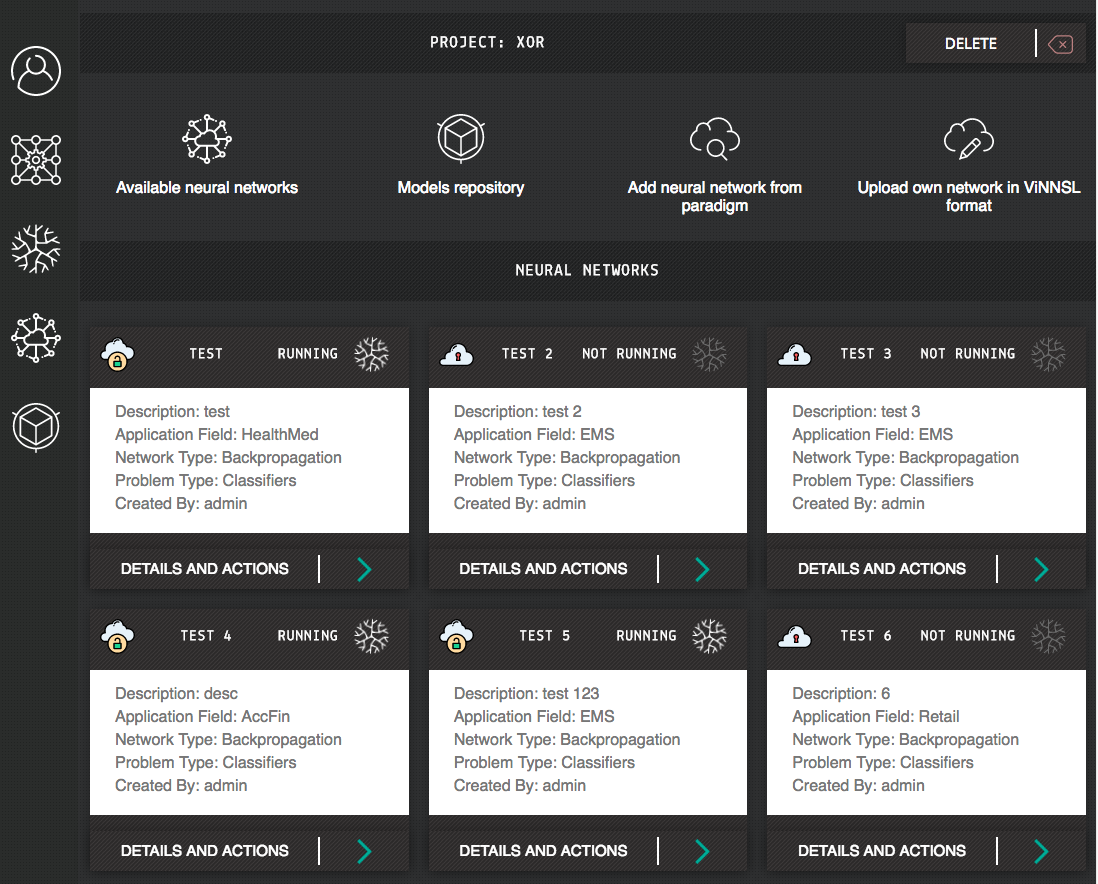
\includegraphics[width=\linewidth]{components/5/img/projects_dsahboard.png}
  \caption{N2Sky User Project Dashboard}
  \label{fig:projects_dsahboard}
\end{center}
\end{figure}

As any other dashboards in N2Sky, the project dashboard contains the available tools and the grid of items.
On the top of the dashboard, the title and the delete button is located. It is possible to delete project only for project owner or system administrator. 

\subsubsection{Available tools.} 

The available tools is a common functionality, which is necessary for project dashboard. Every tool contains an SVG icon and caption underneath as it displayed in figure \ref{ref:projecttools}. 

\begin{figure}[htbp]
\begin{center}
  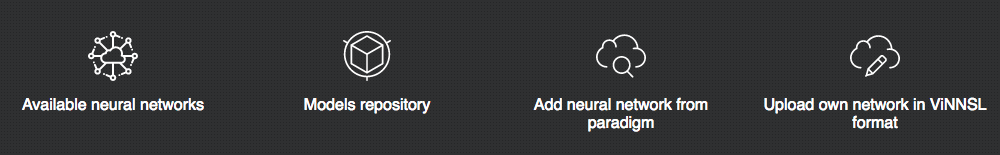
\includegraphics[width=\linewidth]{components/5/img/project_tools.png}
  \caption{N2Sky Project Dashboard. Available tools}
  \label{fig:projecttools}
\end{center}
\end{figure}

The following tools are available for all types of users:
\begin{itemize}
\item \emph{Available neural network.} Reference to the available repositories view.  
\item \emph{Model repository.} Reference to the model repository view.
\item \emph{Add neural network from the paradigm.} Will redirect to the creation of neural network from existing paradigm page. 
\item \emph{Upload own network in ViNNSL format} is mostly used by contributor user since the user needs to know the ViNNSL language. On click, the popup will be initialized as it is shown in figure \ref{fig:upload_vinnsl_popup}. 

\begin{figure}[htbp]
\begin{center}
  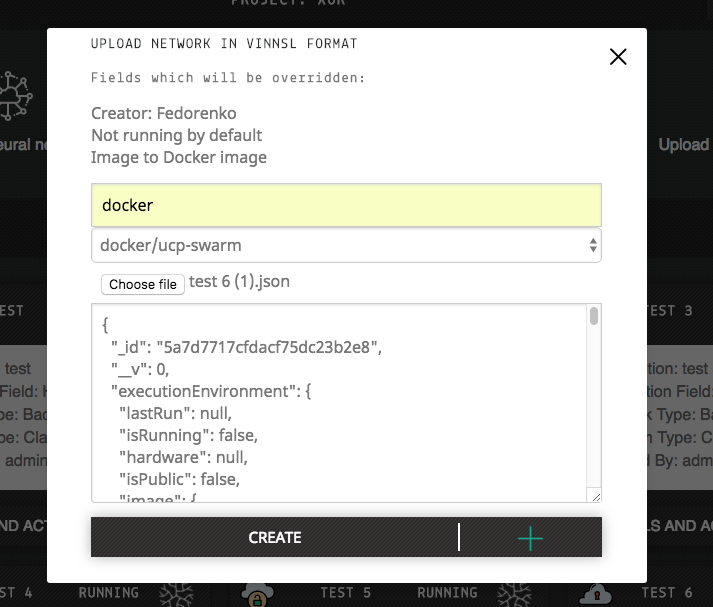
\includegraphics[scale=0.5]{components/5/img/upload_vinnsl_popup.png}
  \caption{N2Sky Project Dashboard.Upload own network in ViNNSL format}
  \label{fig:upload_vinnsl_popup}
\end{center}
\end{figure}

The popup contains following components:
\begin{itemize}
\item The information block about the following operation. The block shows, which fields are going to be overridden namely: the creator field, image information and it will be not running by default. 
\item The Docker username field, which references on the username in Docker Hub repository. After the name will be entered the available images list will be listed. 
\item The Docker image combo box is a list of available images of chosen Docker Hub user.  This image will be used for creating neural network paradigm.
\item The Upload field. The user needs to choose from local machine the neural network paradigm, which is described in ViNNSL XML or JSON format.
\item The text field will show the preview of uploaded neural network paradigm in ViNNSL format.
\item Create button will process the form and create the neural network paradigm. After creation, the user will be redirected to the neural network details page. 
\end{itemize}

\subsubsection{Neural Networks Grid.}

The neural networks grid represents a list all neural network which was created or copied from other users. Every grid item contains brief information about the neural network:
\begin{itemize}
\item The title of the neural network
\item The status tither running or not running. If the instance is running the N2Sky icon will spin, if not it will be grey without movements. 
\item The short description of the neural network
\item Application field
\item Network type
\item Problem type
\item Created by user
\item Details and actions button, which redirect the user to the page with detailed information of the neural network. 
\end{itemize}

\subsubsection{Saved trained models.}

The table with saved trained models is located at the bottom of project dashboard as it is shown in figure \ref{fig:saved_trained_models_project}.

\begin{figure}[htbp]
\begin{center}
  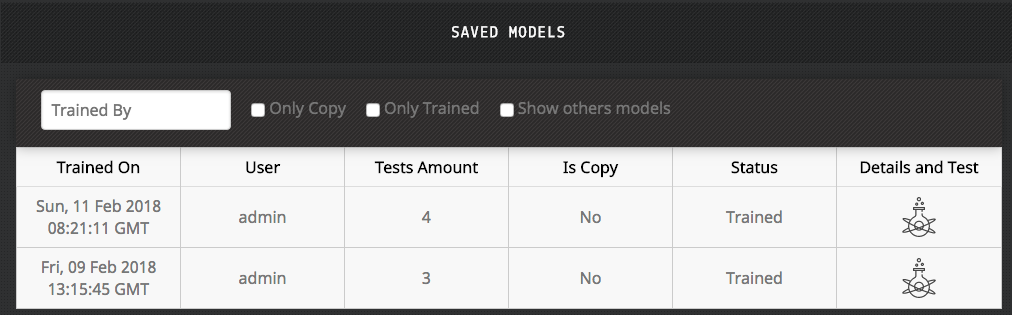
\includegraphics[width=\linewidth]{components/5/img/saved_trained_models_project.png}
  \caption{N2Sky Project Dashboard. Saved trained models}
  \label{fig:saved_trained_models_project}
\end{center}
\end{figure}

This table represents the copied trained models into the particular project. It is possible to perform the semantic search against trained models, the same approach is used in N2Sky Main Dashboard. 

\end{itemize}


\subsection{Three steps view}\label{Three steps view}

Robert Browning in his poem "Andrea del Sarto" said: "Less is mode", which became an inspiration of the "Three steps view". It was derived from the simplicity of the arbitrary user. The idea behind to make possible to create the neural network from the paradigm within only three steps. After creation of the neural network reuse the same three steps to provide the overview of the created neural network.

The following steps have to be achieved in order to create the neural network from the paradigm:  the neural network description, the neural network structure, and the neural network training.

\subsubsection{The Neural Network Description}

When the user just entering to three step view, the fist what he will see it is "The Network Description" tab. In this tab, the user has to choose propagation method which is available on N2Sky. After choosing some propagation method the metadata from the ViNNSL template will be loaded. The metadata is represented as a form as is shown in figure \ref{fig:nn_desc_3_steps}

\begin{figure}[H]
\begin{center}
  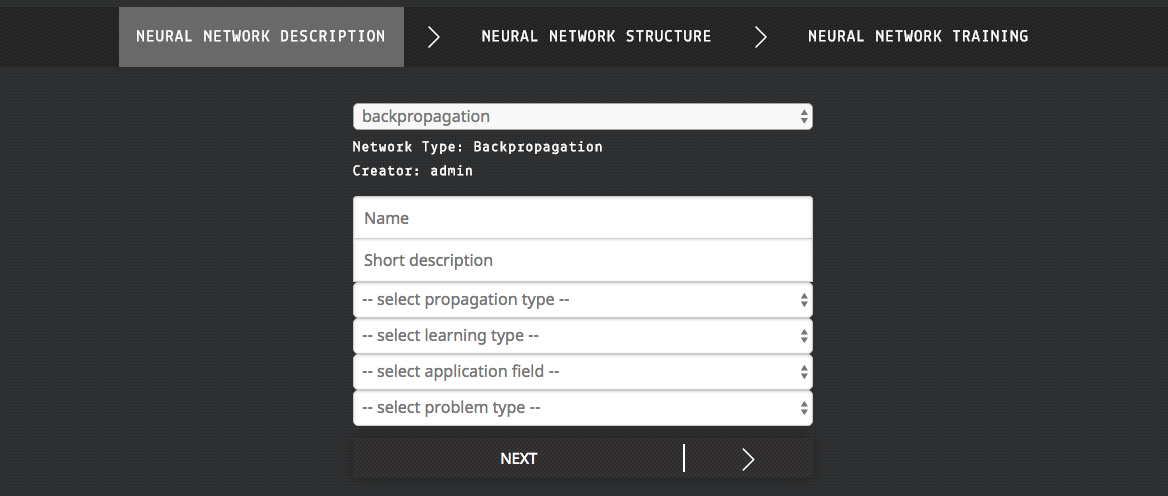
\includegraphics[width=\linewidth]{components/5/img/nn_desc_3_steps.png}
  \caption{Three Steps View. The Neural Network Description}
  \label{fig:nn_desc_3_steps}
\end{center}
\end{figure}

The mandatory metadata from the ViNNSL template is:
\begin{itemize}
\item Name of the neural network
\item Shot description
\item Propagation type
\item Learning type
\item Application field
\item Problem type
\end{itemize}

This data can be customized on demand. Any additional field in metadata of ViNNSL template will be reflected in this form.


After filling up the form, the user will be redirected to the "Neural Network Structure" tab.

\subsubsection{The Neural Network Structure}

The neural network structure field represents the structure of the neural network, which can be customized. It is also possible to set the connections between the layers and nodes. 

When the user entering to this tab he will so only three types of layers: 
\begin{itemize}
\item \emph{Input Layer}, which represents the amount of the nodes in the input layer.
\item \emph{Hidden Layers} can be multidimensional. It has the matrix structure, it means it is possible to choose multiple layers and multiple nodes. The amount of nodes does not have to be equal in each layer.
\item \emph{Output Layer} is a layer, which represents the number of nodes for output. This layer has to validate, because of the difference between neural networks. 
\end{itemize}

After choosing the correct numbers of the layers and nodes the visual representation will be shown as it displayed in figure \ref{fig:nn_structure_3_steps}.


\begin{figure}[htbp]
\begin{center}
  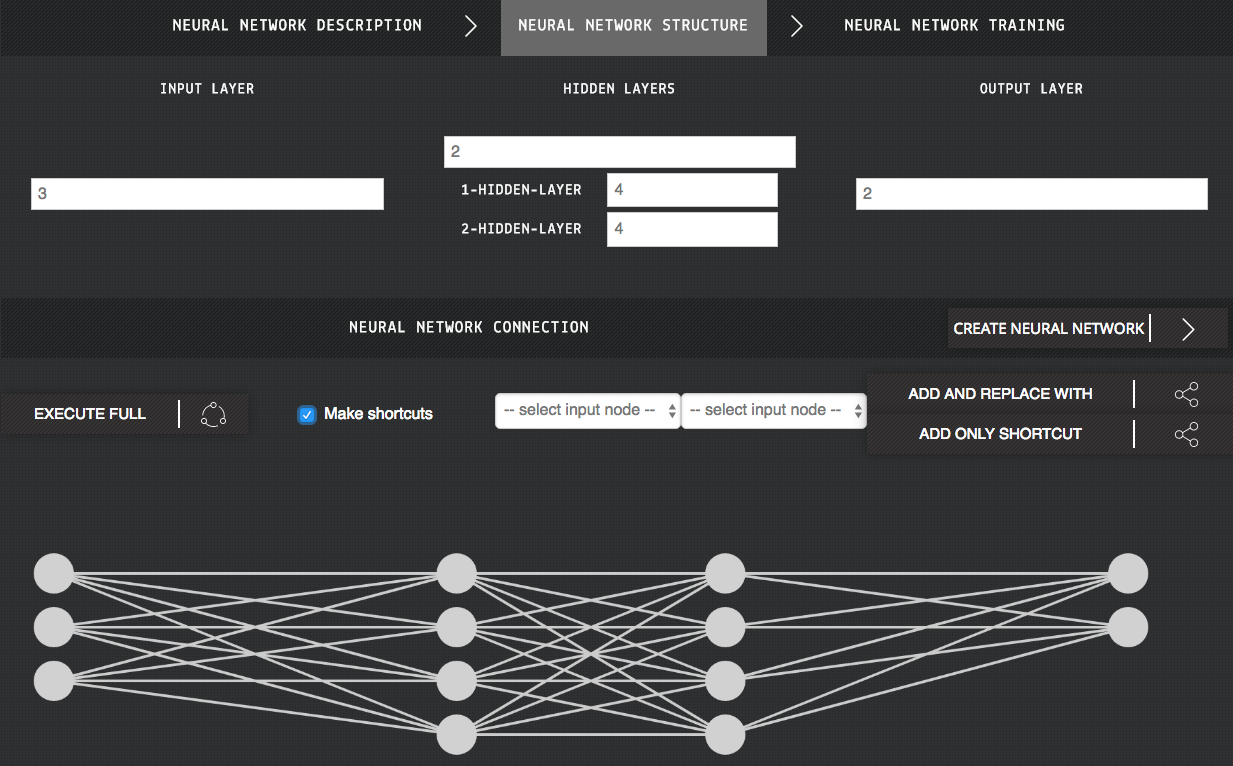
\includegraphics[width=\linewidth]{components/5/img/nn_structure_3_steps.png}
  \caption{Three Steps View. The Neural Network Structure with full connection}
  \label{fig:nn_structure_3_steps}
\end{center}
\end{figure}

The next step is to connect the nodes. Following connections are possible:

\begin{itemize}
\item \emph{Full Connection}. The nodes are full connected when they have the connection to all activation with other layers. This is standard approach in every neural network. The matrix multiplication followed be the bias offset. \cite{nn_connection}. This connection is possible to execute by clicking on "Execute full connection" button as is shown in figure \ref{fig:nn_structure_3_steps}.
\item \emph{Pure Shortcut.} Shortcut connection is also called skip connection. With this connection enables unimpeded information flow. This connection if adding the direct connection to other layers. This approach can gain results by training. \cite{shortcuts_nn} With pure connection it is possible to make some direct connection, it will also remove the full connection to the chosen node.
\item \emph{Only shortcut.} It is the same approach as by pure shortcut, except the full connection still enabled. 
\end{itemize}

In order to make shortcuts connection more understandable, they are will be immediately visualized as is shown in figure \ref{fig:connection_3_steps}. In this example, the first input node has pure shortcut connection with a second hidden layer and the third input node has only shortcut connection with output layer, the gull connection with this node remains the same.

\begin{figure}[htbp]
\begin{center}
  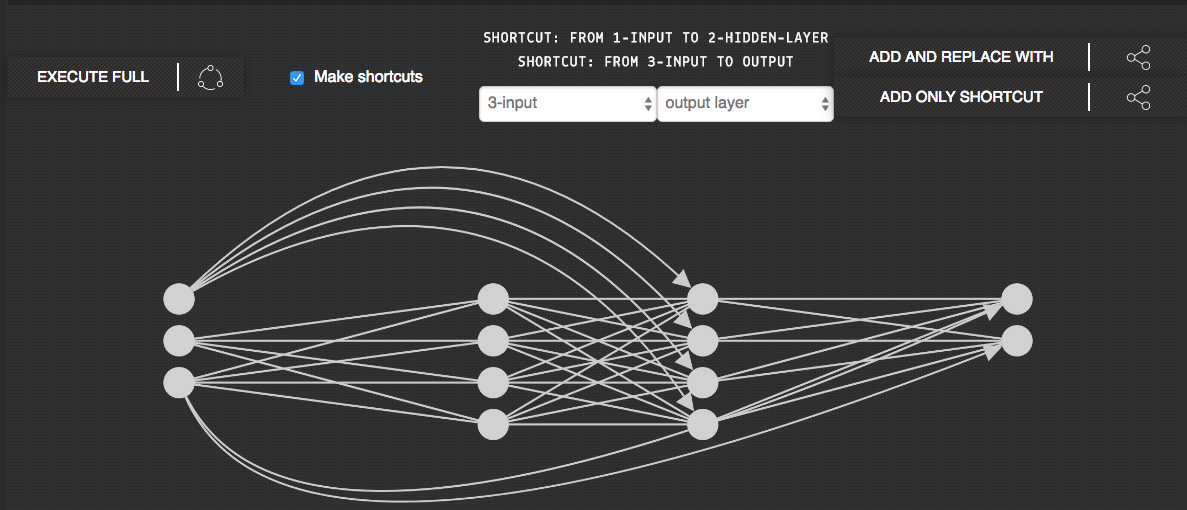
\includegraphics[width=\linewidth]{components/5/img/connection_3_steps.png}
  \caption{Three Steps View. The shortcut connections}
  \label{fig:connection_3_steps}
\end{center}
\end{figure}

After creating the neural network the user will be redirected to the "Neural Network Training" tab. The all other tabs are clickable, but is it not possible to change either metadata or the structure of the neural network.

\subsubsection{The Neural Network Training}

One of the most important steps in three-step view workflow, because from this tab is possible to perform some testing against the newly created neural network. The tab is multifunctional and scalable on permissions of the particular user as is shown in figure \ref{fig:training_3_steps}.

\begin{figure}[H]
\begin{center}
  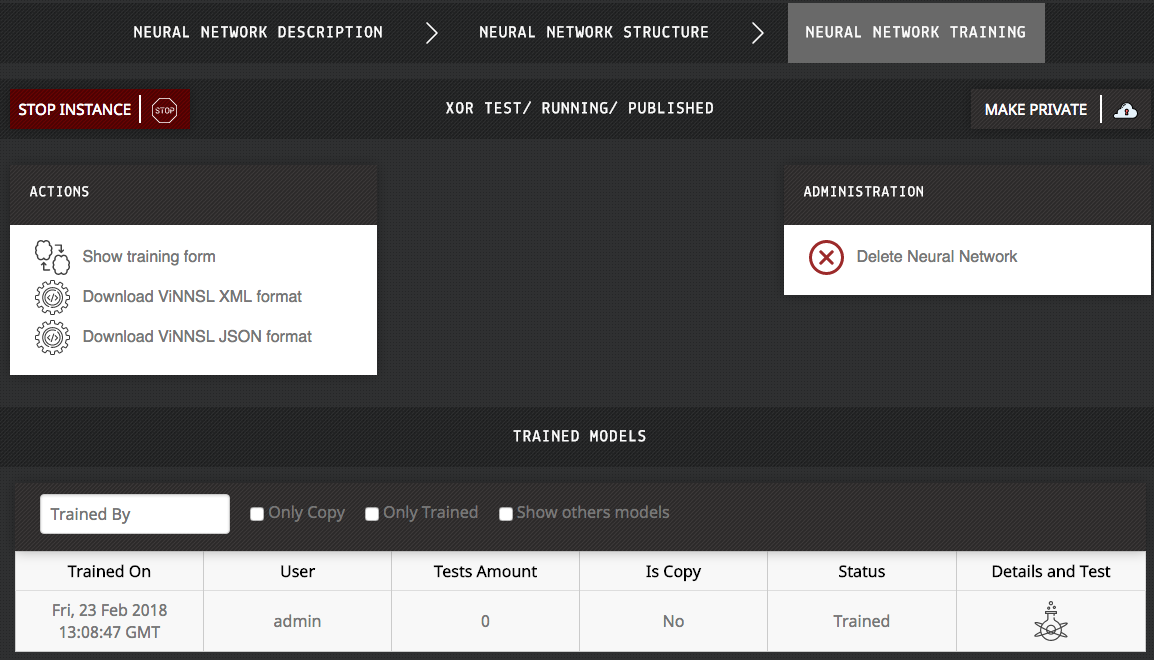
\includegraphics[width=\linewidth]{components/5/img/training_3_steps.png}
  \caption{Three Steps View. The Neural Network Training.}
  \label{fig:training_3_steps}
\end{center}
\end{figure}

There are few components which are available to the user:
\begin{itemize}
\item \emph{Administration.} This block is available only to neural network owner and the system administrator. The following operations are possible to perform from this block:
\begin{itemize}
\item \emph{Run the instance.} Without running the instance it is not possible to perform any testing. The user can run the neural network instance on N2Sky Cloud or if it his own neural network he can deploy on his own publicly available cloud as is shown in figure \ref{fig:run_instance_3_steps}. 

\begin{figure}[H]
\begin{center}
  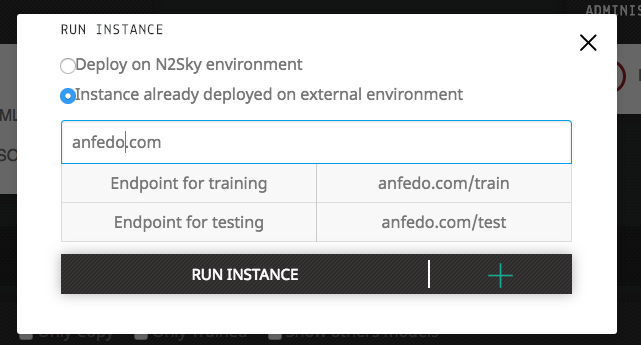
\includegraphics[scale=0.5]{components/5/img/run_instance_3_steps.png}
  \caption{Three Steps View. The Neural Network Training. Run instance}
  \label{fig:run_instance_3_steps}
\end{center}
\end{figure}

Only two endpoints are available:
\begin{itemize}
\item \emph{/train} - for training the neural network. This endpoint has to accept ViNNSL-formatted neural network description and the training data. 
\item \emph{/test} - for evaluating the trained model. Has to accept only testing data.
\end{itemize}
Detailed information of API can be found in Development chapter \autoref{API Documentation}.
\item \emph{Stop the instance.} If the instance is running it is possible to stop it. The instance will be removed from the N2Sky cloud if it was deployed there.
\item \emph{Publish the neural network.} The user can publish running neural network. In this case, the neural network will be available in neural network repository and its trained models also. The other users can copy published neural networks in their own projects. 
\item \emph{Delete the neural network.} If the neural network owner or administrator will decide to remove the neural network, then the all trained models and testing data also will be removed. The neural network will not be published anymore and the running instance will be removed.
\end{itemize}
\item \emph{Actions.} The actions are available for every user if the neural network is published. The following actions can be performed:
\begin{itemize}
\item \emph{Show training form.} On click the training form will be expanded as is shown in figure \ref{fig:expand_training_form}

\begin{figure}[H]
\begin{center}
  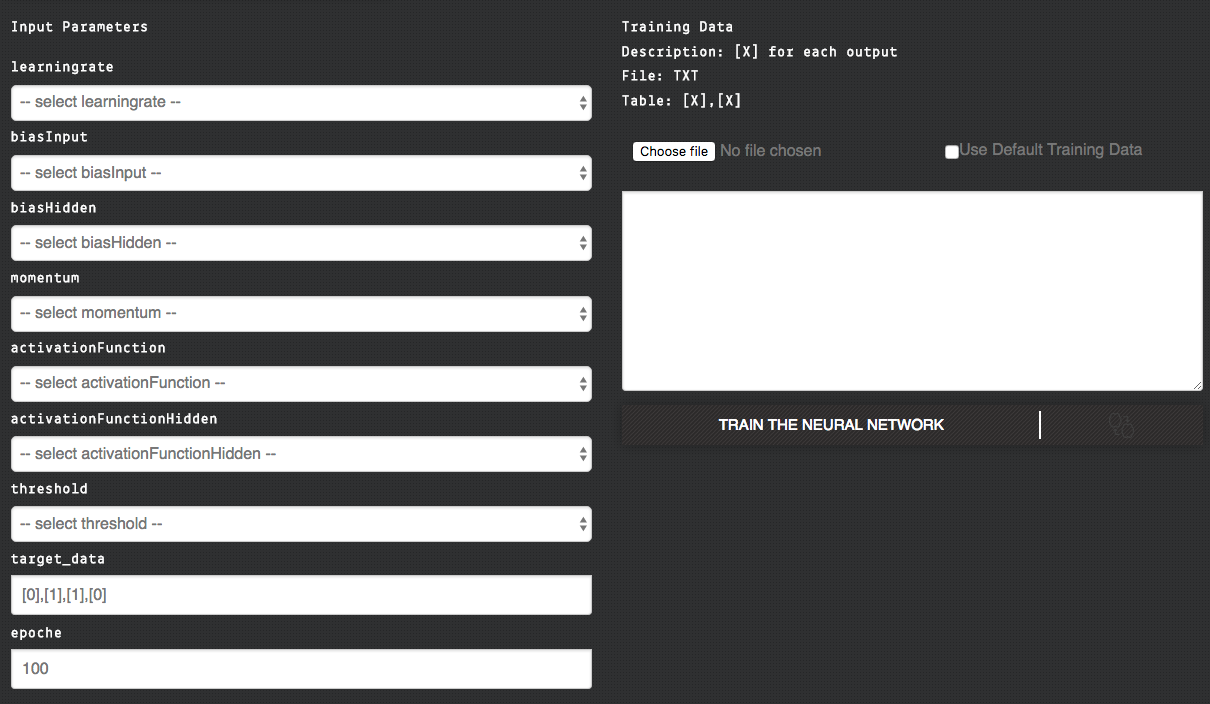
\includegraphics[width=\linewidth]{components/5/img/expand_training_form.png}
  \caption{Three Steps View. The Neural Network Training. Training form}
  \label{fig:expand_training_form}
\end{center}
\end{figure}

The form data is fetched by reflection from ViNNSL Template, namely from input parameters. If there are possible values set in particular the combo box will be shown, if there is only one default value set, the free text field will be displayed.  On the right side, there is training data information box. It is possible to upload own training data or chose default training data.

\item \emph{Download ViNNSL XML format}
\item \emph{Download ViNNSL JSON format}
\end{itemize}

\item \emph{Trained Models Table} is similar to the table in the table in the "Model Repository." It is possible to perform the semantic search against existing trained models. The user can see the status of the training and on the clock of the particular model, he will be redirected to the testing view and detailed information about training.

\end{itemize}

\subsubsection{Training Results and the Model Evaluation}\label{Training results and the model evaluation}

The testing is a part of the model evaluation that is why it is under three-step-view workflow. The training results and the model evaluation page is an underline of the workflow. From this page, the user can observe chosen training model, study the training graph and evaluate trained model as is shown in figure \ref{fig:testing_model}.

\begin{figure}[htbp]
\begin{center}
  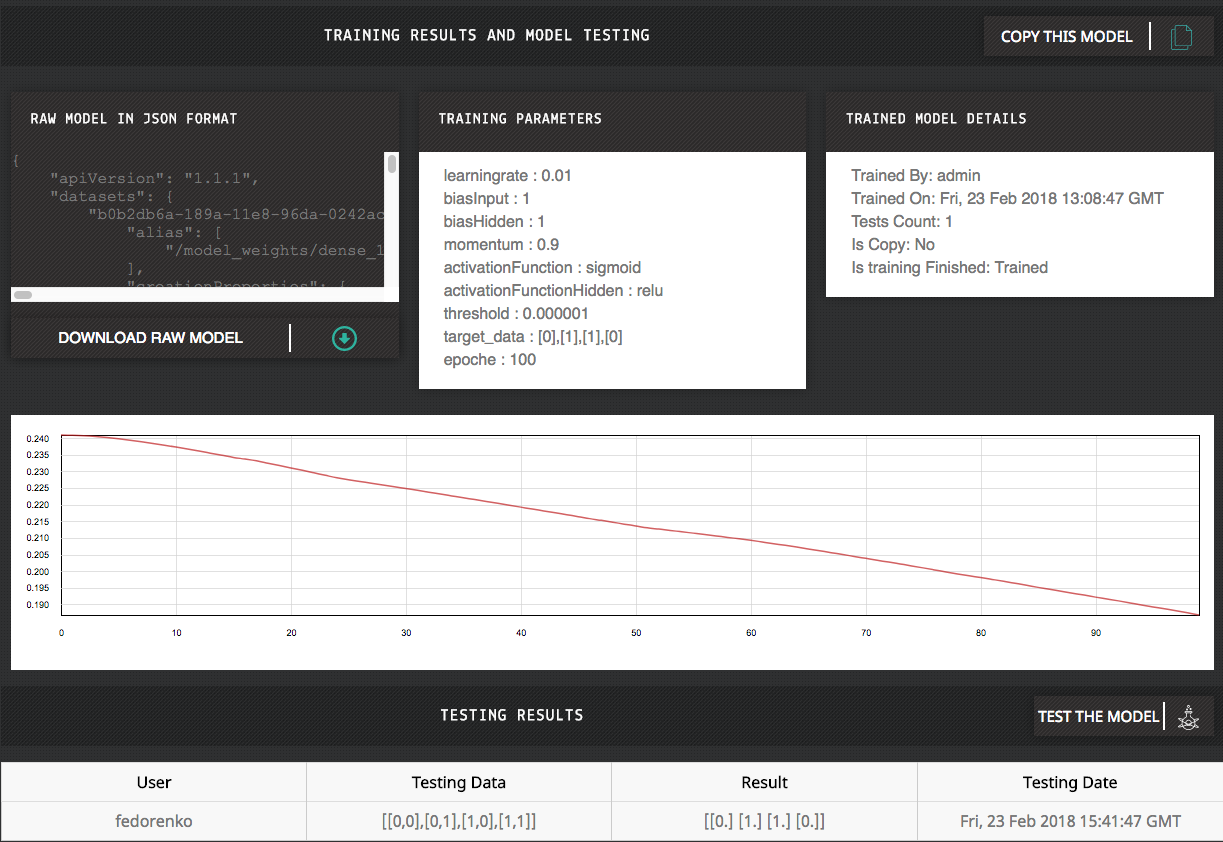
\includegraphics[width=\linewidth]{components/5/img/testing_model.png}
  \caption{Three Steps View. Training Results and the Model Evaluation}
  \label{fig:testing_model}
\end{center}
\end{figure}

The page view contains following elements:
\begin{itemize}
\item \emph{Functional bar} consists of the title itself and the functional copy of the project button. The functionality is pretty the same as copying the neural network to the own project from the neural network repository. The user has to choose the project in popup modal window and then perform copying as is shown in figure \ref{fig:copy_model}. It is possible to copy the trained model into multiple projects. 

\begin{figure}[htbp]
\begin{center}
  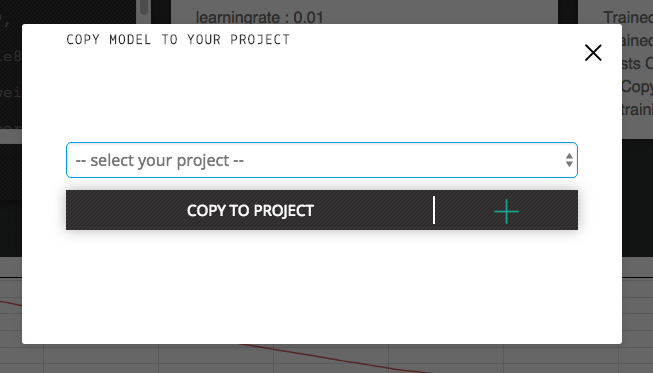
\includegraphics[scale=0.5]{components/5/img/copy_model.png}
  \caption{Three Steps View. Training Results and the Model Evaluation. Copy model into own project.}
  \label{fig:copy_model}
\end{center}
\end{figure}

\item \emph{Row model in JSON format}, which gives an overview of the trained model. The model can be viewed directly from UI as well as it is possible to download it and review from Desktop or mobile device. 
\item \emph{Training parameters} is the input parameters, with which the neural network was trained. The parameters can differentiate from paradigm to paradigm.
\item \emph{Trained model detail} is the metadata of the trained model. Namely, timestamp event metadata information. It contains following data:
\begin{itemize}
\item Trained by user information
\item Trained on timestamp
\item Tests count (the tests, which are already performed)
\item Is a copy information
\item Is training finished information
\end{itemize}

\item \emph{Graph}, which represents epochs in x-axis and error on the y-axis. If the neural network still in process of the training the graph will move with it. 
\item \emph{Test the model} button will initiate the testing popup modal window as is shown in figure \ref{fig:model_testing}. The user has to choose the testing data, it is possible to use the default values.

\begin{figure}[htbp]
\begin{center}
  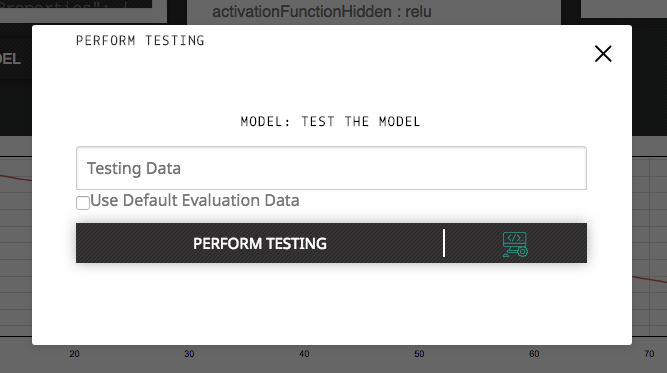
\includegraphics[scale=0.5]{components/5/img/model_testing.png}
  \caption{Three Steps View. Training Results and the Model Evaluation. The model testing.}
  \label{fig:model_testing}
\end{center}
\end{figure}

\item \emph{Testing results} it a table with testing results. The user can see only his own testing results if the user is the neural network owner or the system administrator he can see the results from other users also. The table has following columns:
\begin{itemize}
\item The user who performs the testing 
\item The testing data
\item Results (output)
\item Testing Date
\end{itemize}


\end{itemize}





\subsection{Neural Networks Repository}\label{Neural Networks Repository}

The neural repository is representing a repository, where any user can find and reuse available neural network. The neural network repository contains the search bar and the grid with the published neural networks as it displayed in figure \ref{fig:nn_repository}. If the neural network is published by the neural network owner, it is automatically added to the repository. It is important to mention, that only published networks of other users will be displayed. 

\begin{figure}[H]
\begin{center}
  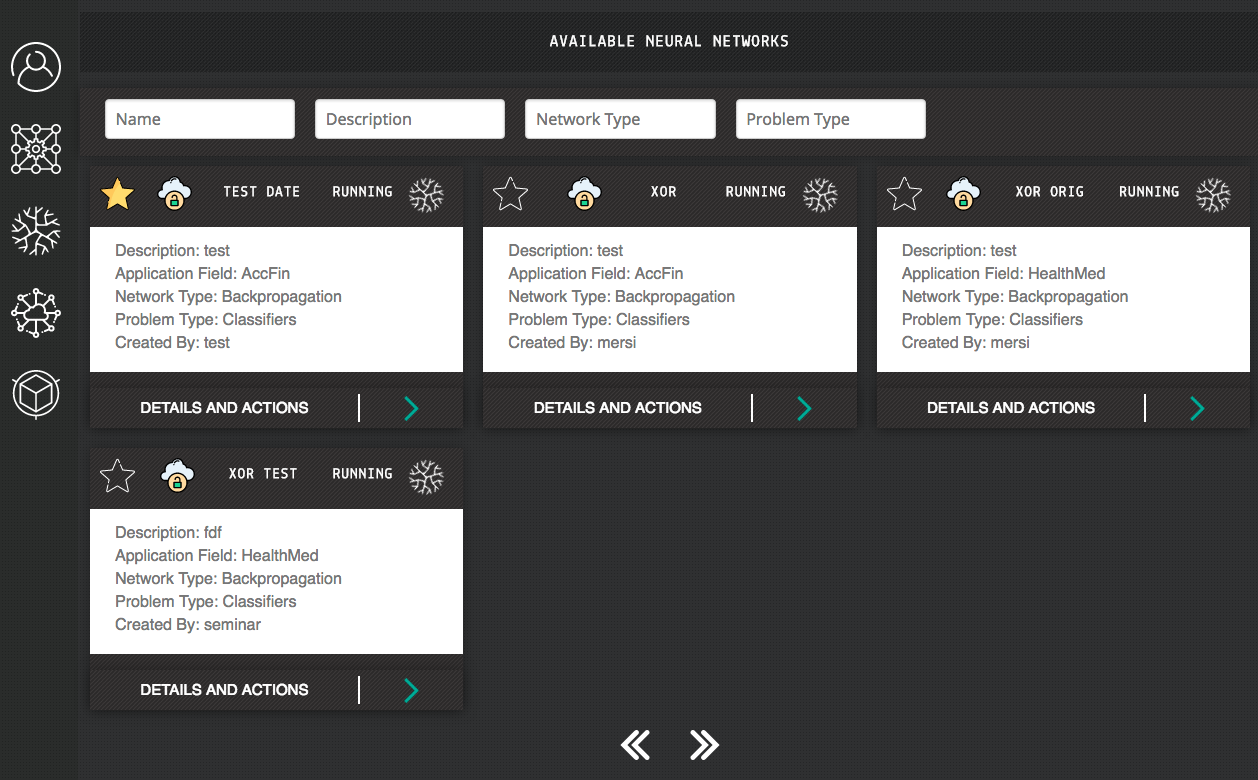
\includegraphics[width=\linewidth]{components/5/img/nn_repository.png}
  \caption{N2Sky Neural network repository}
  \label{fig:nn_repository}
\end{center}
\end{figure}


\begin{enumerate}
\item \emph{Searching bar.} With the searching bar is possible to perform the semantic search against available neural networks in the repository. It is possible to search by: 
\begin{itemize}
\item Name of the neural network
\item Description of the neural network
\item Network Type
\item Problem Type
\end{itemize}

Each field is case insensitive. The inquiry will be processed in converted in order to give most reliable results. 

\item \emph{Networks grid} is a grid, which represents the published neural networks. It has 3 columns in Desktop version and 1 in the mobile version. Every grid item has a title, which contains following components:
\begin{itemize}
\item The save button-icon. The button is displayed as a start. If the star has a color then the neural network already saved. If the icon is transparent it means that it is possible to save the neural network. On click of the transparent button, the popup modal window will appear as is shown in figure \ref{fig:copy_nn}. From the modal window, the user can choose available projects, where he can copy chosen neural network. 


\begin{figure}[htbp]
\begin{center}
  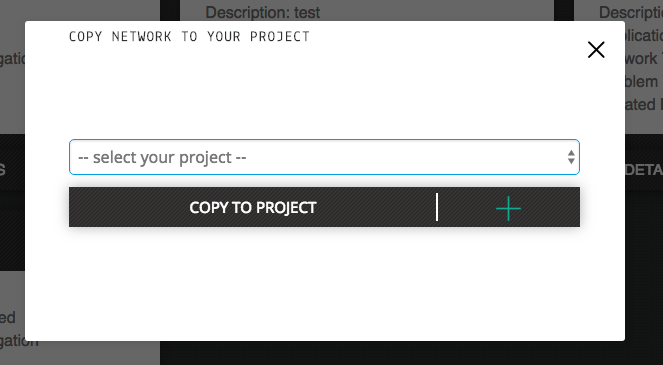
\includegraphics[scale=0.5]{components/5/img/copy_nn.png}
  \caption{N2Sky Neural network repository. Copy the neural network.}
  \label{fig:copy_nn}
\end{center}
\end{figure}

\item Availability of the neural network. Can be public (green), private (red) and restricted (yellow). The arbitrary user can observer only public neural networks, the administrator can observe any neural network in N2Sky.  

\item The name of the neural network
\item The running status. Can be running and not running.
\item The running icon. Can be spinning icon for running and standing alone is for not running the network.
\end{itemize}

Besides details and actions button, which redirect the user to neural network details, the brief network information is deployed:
\begin{itemize}
\item Short description
\item Application field
\item Network type
\item Problem type
\item Created by
\end{itemize}

\end{enumerate}

\subsection{Models Repository}\label{Models Repository}

The modal repository is similar to neural networks repository but contains only trained models. The structure is also different. Because of the big amount of the trained models the models are displayed in the table as is shown in figure \ref{fig:model_repo}. 

\begin{figure}[H]
\begin{center}
  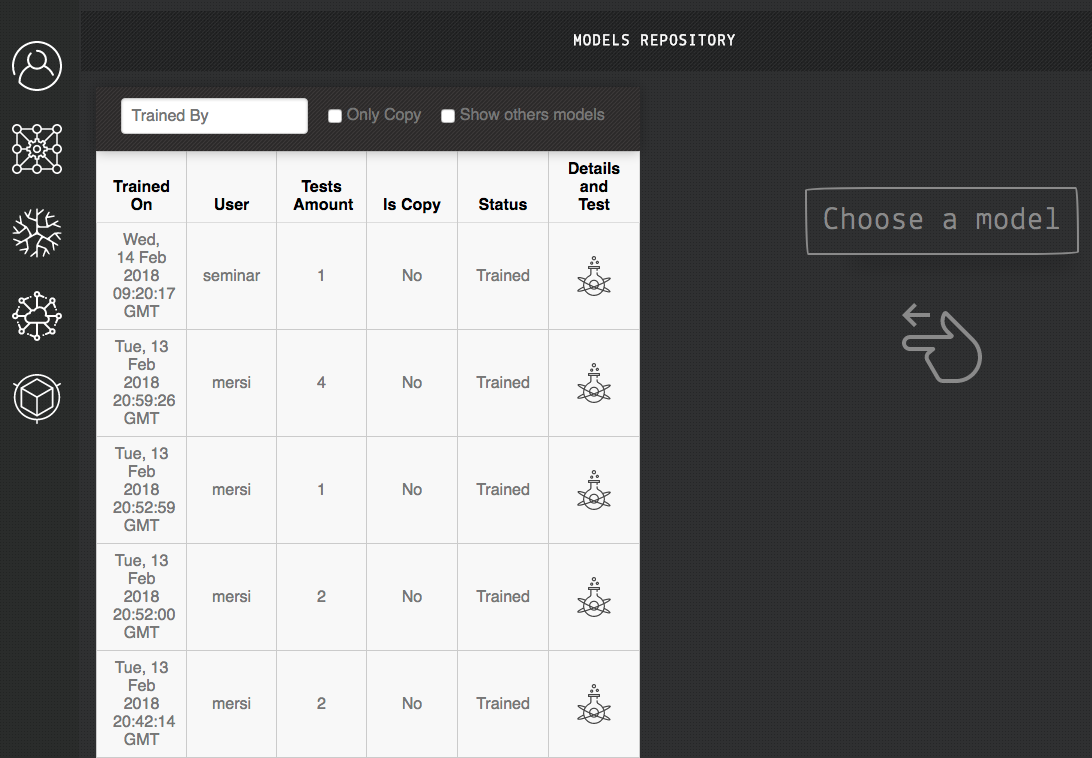
\includegraphics[width=\linewidth]{components/5/img/model_repo.png}
  \caption{N2Sky Models Repository}
  \label{fig:model_repo}
\end{center}
\end{figure}

The model repository page view contains models table and a brief description of  the chosen model:
\begin{itemize}
\item \emph{Trained model table} is consist of the search bar and table itself.
\begin{itemize}
\item The search bar gives possibility perform the semantic search against available trained models. It has following filters:
\begin{itemize}
\item Trained by
\item Only copy checkbox
\item Show other models checkbox
\end{itemize}
\item The table. On clock of the table, the short description of the trained model will be opened. The table contains following elements:
\begin{itemize}
\item Trained on (timestamp)
\item User
\item Tests amount
\item Is copy
\item Status
\item Details and tests
\end{itemize}
\end{itemize}

\item \emph{The short description} is located on the right side of the page. When the user just entering to the page there will be only notification, which motivates the user to chose the model. After choosing it, the view will be replaced with a short description as is shown in figure \ref{fig:short_desc}.

\begin{figure}[H]
\begin{center}
  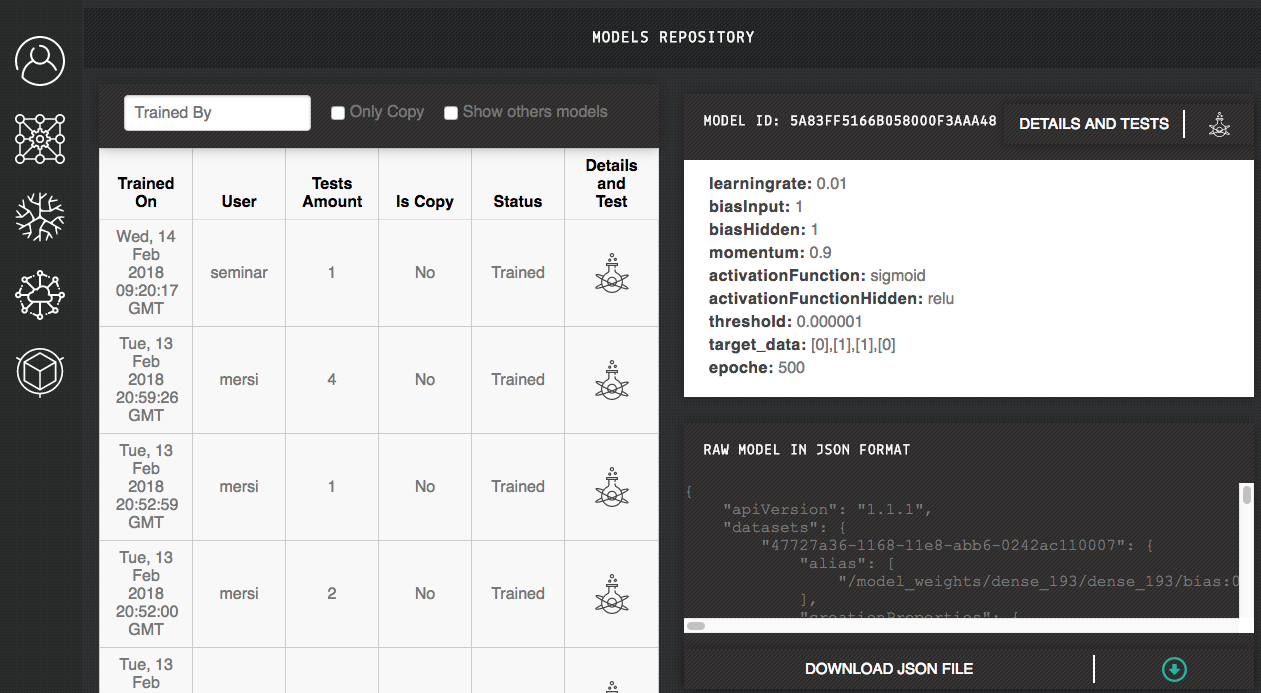
\includegraphics[width=\linewidth]{components/5/img/short_desc.png}
  \caption{N2Sky Models Repository. Short Description}
  \label{fig:short_desc}
\end{center}
\end{figure} 

The description contains following components:
\begin{itemize}
\item Title, which consists of the ID of the model and button, which will redirect to details of the chosen model.
\item The list of the input parameters. This list can differ, depending on neural network paradigm. 
\item The raw model, which can be downloaded. 
\end{itemize}

\end{itemize}
